The simplest way of evaluating a derivative is by computing the difference between the evaluation of the function at a given point and a small perturbation of the function. 
In the case of a loss function, we can approximate
\begin{equation}
 \frac{dL}{d\theta_i} (\theta) \approx \frac{L(\theta + \varepsilon e_i ) - L(\theta)}{\varepsilon},
 \label{eq:finite_diff}
\end{equation}
with $e_i$ the $i$-th canonical vector and $\varepsilon$ the stepsize. 
Even better, it is easy to see that the centered difference scheme
\begin{equation}
 \frac{dL}{d\theta_i} (\theta) \approx \frac{L(\theta + \varepsilon e_i ) - L(\theta - \varepsilon e_i)}{2\varepsilon},
 \label{eq:finite_diff2}
\end{equation}
leads also to more precise estimation of the derivative. 
While Equation \eqref{eq:finite_diff} gives to an error of magnitude $\mathcal O (\varepsilon)$, the centered differences schemes improves to $\mathcal O (\varepsilon^2)$. 
 
However, there are a series of problems associated to this approach.
The first one is due to how this scales with the number of parameters $p$.
Each directional derivative requires the evaluation of the loss function $L$ twice.
For the centered differences approach in Equation \eqref{eq:finite_diff2}, this requires a total of $2p$ function evaluations, which at the same time demands to solve the differential equation in forward mode each time for a new set of parameters.

A second problem is due to rounding errors.
Every computer ultimately stores and manipulate numbers using floating points arithmetic \cite{Goldberg_1991_floatingpoint}. 
Equations \eqref{eq:finite_diff} and \eqref{eq:finite_diff2} involve the subtraction of two numbers that are very close to each other, which leads to large cancellation errors for small values of $\varepsilon$ than are amplified by the division by $\varepsilon$.
On the other hand, large values of the stepsize give inaccurate estimations of the gradient. 
Finding the optimal value of $\varepsilon$ that trade-offs these two effects is sometimes called the \textit{stepsize dilemma} \cite{mathur2012stepsize-finitediff}.
Due to this, some heuristics and algorithms had been introduced in order to pick the value of $\varepsilon$ that will minimize the error \cite{BARTON_1992_finite_diff, mathur2012stepsize-finitediff}, but all these methods require some a priori knowledge about the function to be differentiated. 
If well many analytical functions, like polynomials and trigonometric functions, can be computed with machine precision, numerical solutions of differential equations have errors larger than machine precision, which leads to inaccurate estimations of the gradient when $\varepsilon$ is too small. 
This is illustrated in Figure \ref{fig:finite-diff}, where the error in computing the gradient is shown for both true analytical solution and numerical solution of a system of ODEs as a function of the stepsize.

% Condition error
%specifically picking $\varepsilon^* = \sqrt{\varepsilon_\text{machine}} \| \theta \|$, with $\varepsilon_\text{machine}$ the machine precision (e.g. \texttt{Float64}).
 
% Even with all these caveats, finite differences can be useful when computing Jacobian-vector products. Suppose we are interested in computing 
% \begin{equation}
% \frac{du}{d\theta} v, 
% \end{equation}
% with $v \in \mathbb R^p$ a vector. This last evaluation corresponds to the directional derivative in the direction of $v$. Then, we can save some computations by directly computing the Jacobian-vector product as 
% \begin{equation}
% \frac{dL}{d\theta} v \approx \frac{L(\theta + \varepsilon v) - L(\theta - \varepsilon v)}{2\varepsilon},
% \end{equation}
% which depending on the output size of the function $L(\theta)$, could be a reasonable idea. 

Replacing derivatives by finite differences is also a common practice when solving partial differential equations (PDEs), a technique known as the \textit{method of lines} \cite{ascher2008numerical}. 
To illustrate this point, let us consider the case of the one-dimensional heat equation
\begin{equation}
 \frac{\partial u}{\partial t}
 = 
 D \, 
 \frac{\partial^2 u}{\partial x^2}, 
 \quad u(0, t) = \alpha(t), 
 \quad u(1, t) = \beta(t)
 \label{eq:heat-equation}
\end{equation}
that includes both spatial and temporal partial derivatives of the unknown function $u(x, t)$.
In order to numerically solve this equation, we can define a spatial grid with coordinates $m \Delta x$, $m=0, 1, 2, \ldots, N$ and $\Delta x = 1 / N$.
If we call $u_m(t) = u(m \Delta x, t)$ the value of the solution evaluated in the fixed points in the grid, then we can replace the second order partial derivative in Equation \eqref{eq:heat-equation} by the corresponding second order finite difference\footnote{Since $u_m(t)$ is a function of one single variable, we write the total derivative $\frac{du_m}{dt}$ instead of the partial derivative symbol used before $\frac{\partial u}{\partial t}$, which it is usually used just for multivariable function.}
\begin{equation}
 \frac{d u_m}{dt} 
 = 
 D 
 \frac{u_{m-1} - 2u_m + u_{m+1}}{\Delta x^2}
 \label{eq:heat-equation-discrete}
\end{equation}
for $m = 1, 2, \ldots, N-1$ (in the extremes we simply have $u_0(t) = \alpha(t)$ and $u_N(t)=\beta(t)$).
Now, equation \eqref{eq:heat-equation-discrete} is a system of ordinary differential equations (just temporal derivatives) with a total of $N-1$ equations.
This can be solved directly using an ODE solver.
Further improvements can be made by exploiting the fact that the coupling between the different functions $u_m$ is sparse, that is, the temporal derivative of $u_m$ just depends of the values of the function in the neighbour points in the grid.

\begin{figure}[tbh]
    \centering
    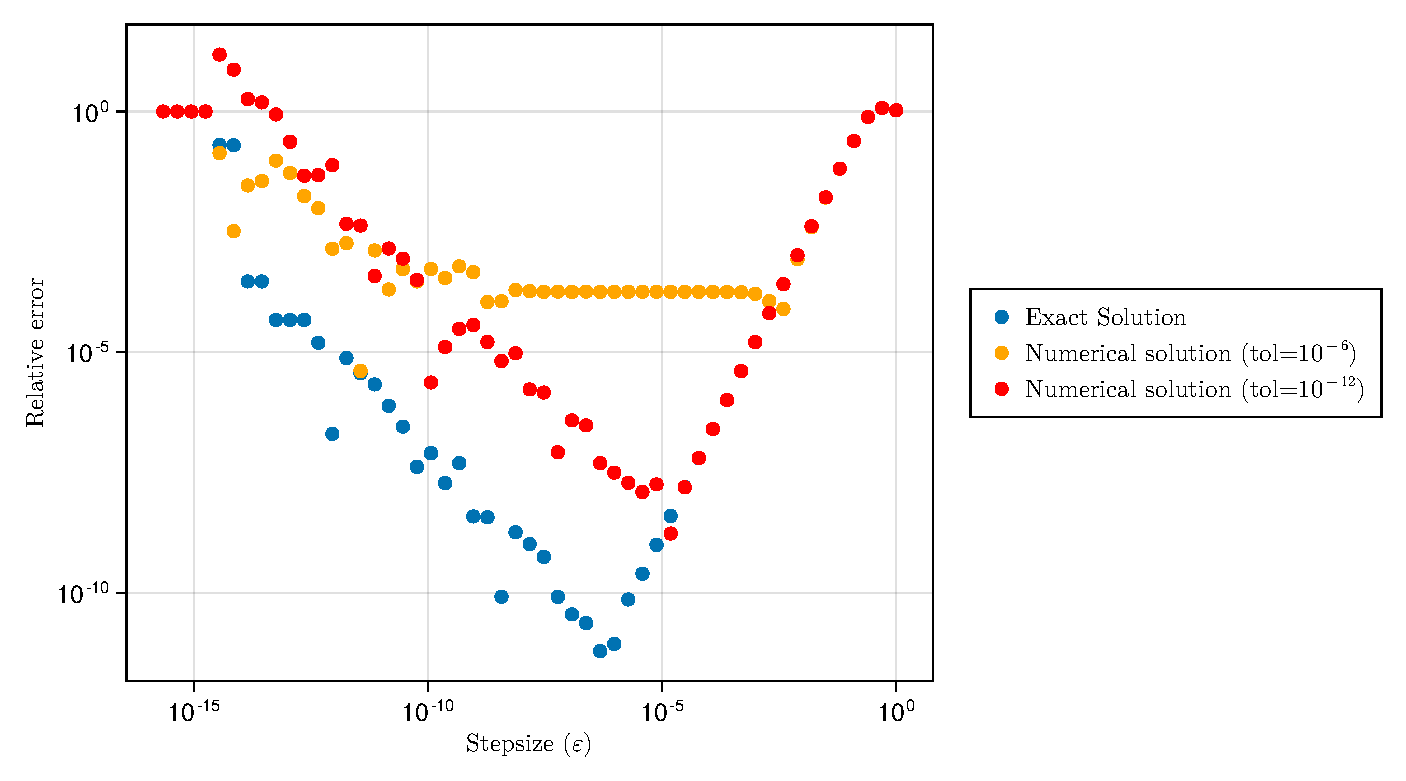
\includegraphics[width=0.85\textwidth]{../code/finite_differences/finite_difference_derivative.pdf}
    \caption{Absolute relative error when computing the gradient of the function $u(t) = \sin (\omega t)/\omega$ with respect to $\omega$ at $t=10.0$ as a function of the stepsize $\varepsilon$. Here $u(t)$ corresponds to the solution of the differential equation $u'' + \omega^2 u = 0$ with initial condition $u(0)=0$ and $u'(0)=1$. The blue dots correspond to the case where this is computed finite differences. The red and orange lines are for the case where $u(t)$ is numerically computed using the default Tsitouras solver \cite{Tsitouras_2011} from \texttt{OrdinaryDiffEq.jl} using different tolerances. The error when using  a numerical solver is larger and it is dependent of the numerical precision of the numerical solver. }
    \label{fig:finite-diff}
\end{figure}